%\documentclass[11pt,hyperref={bookmarks=false}]{beamer}
%\documentclass[11pt,handout]{beamer}
\documentclass[11pt]{beamer}
%\usetheme{Copenhagen}
%\usetheme{default}
\usetheme{default}
%\usecolortheme{seagull}
\usefonttheme{professionalfonts}
%\useoutertheme{infolines}%{miniframes}
%\usepackage{xmpmulti}
%\usepackage{latexsym,fancyhdr,array,tabularx,multicol}
%\usepackage{ifthen,booktabs,calc,longtable,lscape,amsmath}
%\usepackage{egameps}
% \usepackage[usenames,dvipsnames]{pstricks}
% \usepackage{epsfig}
% \usepackage{pst-grad} % For gradients
% \usepackage{pst-plot} % For axes
%\usepackage{psfrag,graphicx}
\usepackage{graphicx,xfrac}
%\usepackage{xmpmulti}
\usepackage{latexsym,fancyhdr,array,tabularx,multicol,multirow}
\usepackage{booktabs}
\usepackage{amsmath}
%\usepackage{multicol,ifthen,calc}
%\usepackage{multirow}
%\usepackage{pgf}
%\usepackage{longtable, lscape}
%\usepackage{lscape}
\newtheorem{df}{Definition}
\newtheorem{lm}{Lemma}
\newtheorem{prp}{Proposition}
\newtheorem{sprf}{Sketch of Proof}
\newtheorem{prf}{Proof}
\newtheorem{conjecture}{Conjecture}
\newtheorem{suffc}{Sufficient Condition}
\setbeameroption{hide notes}
%\newcommand{\threelinebracer}{$\left. \begin{array}{c} \\ \\ \\ \end{array} \right\rbrace$}
%\newcommand{\threelinebracel}{$\left. \begin{array}{c} \\ \\ \\ \end{array} \right\lbrace$}
%\newcommand{\twolinebracer}{$\left. \begin{array}{c} \\ \\ \end{array} \right\rbrace$}
%\newcommand{\twolinebracel}{$\left. \begin{array}{c} \\ \\ \end{array} \right\lbrace$}
\linespread{1.1}
%\setlength{\parindent}{0pt}
\usepackage{parskip}
\addtolength{\parskip}{0pt}
%\newenvironment{num}
% {\leftmargini=6mm\leftmarginii=8mm
%  \begin{itemize}}{\end{itemize}}
% Separate slides by \begin{frame} and \end{frame}.
\title{The Allocation of Teaching Talent and Human Capital Accumulation}
\author[shortname]{Simeon Alder\inst{1} \and Yulia Dudareva\inst{1} \and Ananth Seshadri\inst{1}}
\institute[shortinst]{\inst{1} University of Wisconsin--Madison}
\date{}
\begin{document}

\begin{frame}
\titlepage
\end{frame}

%\begin{frame}
%\frametitle{Introduction}
%\begin{itemize}
%  \item Public education in U.S. has gone through major (positive) changes since end of WW II, e.g.
%\begin{itemize}
%  \item Real expenditures per student per year: \$2,100 (1950s) to \$12,000 (2010s)
%  \item Student-teacher ratio: 27 (1955) to 16 (2010s)
%\end{itemize}
%
%  \item At same time, educational outcomes don't compare favorably with other developed countries.
%
%  \item Potential explanations include:
%\begin{itemize}
%  \item Local funding for public education (property taxes)
%  \item Role of (powerful) teachers' unions \pause
%  \item \alert{Occupational choice}
%\end{itemize}
%
%\end{itemize}
%
%\end{frame}
%
%\begin{frame}
%\frametitle{Introduction (cont'd)}
%\begin{itemize}
%  \item Broad labor market facts and trends are consistent with occupational choice as a key mechanism:
%  \begin{itemize} \pause
%  \item Female educational attainment rising
%  \item Female labor force participation rising
%  \item Labor market discrimination against women declining
%  \item U.S. public school teachers largely female
%\end{itemize} \pause
%  \item Static losses vs. dynamic gains
%\end{itemize}
%\end{frame}

\begin{frame}
\frametitle{Model}
\framesubtitle{Endowments, Preferences}
\begin{itemize}
  \item Each period, a measure $M$ of agents is born and lives for two periods (``young'' and ``old'')
  \item Individuals born with occupation-specific abilities drawn from a joint bivariate Fr\'echet distribution with c.d.f.
  \begin{equation*}
\label{ }
F(a^T,a^O) = \exp \left[ - a_T^{-\theta} - a_O^{-\theta} \right],
\end{equation*}
%  \item Individuals live for two periods labeled ``young'' and ``old'' and economy populated by two overlapping generations
  \item Individuals have $\log$ preferences over leisure and consumption (no discounting)
\end{itemize}
\end{frame}

\begin{frame}
\frametitle{Model}
\framesubtitle{Technologies}
\begin{itemize}
  \item Children (``young'') make occupation-specific educational investments (in units of time and output)
  \item Adults work as \alert{teachers} or \alert{production workers}.
  \item Technologies are occupation-specific:
  \begin{description}
  \item[Human capital production] (teaching) depends on teacher's $h^T$, child's ability $a$, and child's educational investments (time $s$ and goods $e$) according to:
  \begin{align*}
\label{}
h^{'}(a) & = \left( h^T\right)^\beta a^\alpha s\left(a\right)^\phi e(a)^\eta {N(h^T,\widetilde{H^T})}^{-\sigma}
\end{align*}
  \item[Final output production] depends on adult worker's human capital $h^O$ and exogenous productivity $A^O$:
    \begin{align*}
\label{}
y = A^O h^O
\end{align*}
\end{description}
\end{itemize}
\end{frame}


\begin{frame}
\frametitle{Model}
\framesubtitle{Values}
\begin{align*}
V^g(a^T,a^O,\widetilde{H}^T) & = \max_{\{s^{O},s^{T},e^{O},e^{T}\}} \bigg\{ V^{O,g}(a^O,\widetilde{H}^T), V^{T,g}(a^T,\widetilde{H}^T) \bigg\}
\end{align*}
where
\begin{align*}
%\label{eq:vo}
V^{O,g}(a^O,\widetilde{H}^T) & = \ln\left(1-s^O\left(a^O,\widetilde{H}^T\right)\right) \\
& + \mu \ln \Big[ {{h'}^{O}} {A'}^O(1-{{\tau'}^{O,g,w}})\alert{(1-t)} \\
& - e^O(a^O,\widetilde{H}^T)(1+\tau^{O,g,e}) \Big],  \\
%\label{eq:vt}
V^{T,g}(a^T,\widetilde{H}^T) & = \ln\left(1-s^T\left(a^T,\widetilde{H}^T\right)\right)  \\
& + \mu \ln \Big[ \omega'({{h'}^{T}},{\widetilde{H'}^{T}})(1-{{\tau'}^{T,g,w}})\alert{(1-t)}  \\
& - e^T(a^T,\widetilde{H}^T)(1+\tau^{T,g,e}) \Big] 
\end{align*}
\end{frame}

\begin{frame}
\frametitle{Model (cont'd)}
\framesubtitle{Constraints, Laws of Motion}
\begin{align}
%H^{T} & = \int_{0}^{\infty} \left(h^{T}(a)\right)^{\frac{\beta}{\sigma}} f^{T}(a) da \\
T & = \int_0^\infty \omega\left(h^{T'}(a)\right) {f'}^T(a) da \nonumber\\%\frac{2}{M} \int_0^\infty \omega\left(h^{T'}(a)\right) {f'}^T(a) da \nonumber\\
%\label{eq:densT}
f^T(a) & = \int_0^{\bar{a}^{-1}\left(a\right)} f\big(a,b \big) db \nonumber\\
%\label{eq:densO}
f^O(b) & = \int_0^{\bar{a}\left(b\right)} f\big(a,b \big) da \nonumber
%f^T(a) & = \int_0^{\bar{a}\big(a;H^T,{H^T}'\big)} f\big(a,a^O\big) da^O 
\end{align}
Aggregate laws of motion for $\widetilde{H}^T$ and ${H}^O$:
\begin{align}
%\label{eq:lomT}
\widetilde{H'}^{T} & = \int_0^\infty \left(\left(\tfrac{2 \widetilde{H}^T}{M}\right)^\sigma a^\alpha s^T\left(a,\widetilde{H}^T\right)^\phi e^T(a,\widetilde{H}^T)^\eta \right)^{\frac{\beta}{\sigma}} f^T(a) da \nonumber \\
%\label{eq:lomO}
{H'}^{O} & = \int_0^\infty \left(\tfrac{2 \widetilde{H}^T}{M}\right)^\sigma a^\alpha s^O\left(a,\widetilde{H}^T\right)^\phi e^O(a,\widetilde{H}^T)^\eta  f^O(a) da \nonumber
\end{align}
\end{frame}

\begin{frame}
\frametitle{Model (cont'd)}
\framesubtitle{Occupational Threshold}
%Idiosyncratic human capital investment technology:
%\begin{align*}
%\label{}
%h^{O'}(a^O) & = \left(\frac{2 H^T}{M}\right)^\sigma \left(a^O\right)^\alpha s^O\left(a^{O},H^T,{H^T}'\right)^\phi e^O(a^{O},H^T,{H^T}')^\eta \\
%h^{T'}(a^T) & = \left(\frac{2 H^T}{M}\right)^\sigma \left(a^T\right)^\alpha s^T\left(a^{T},H^T,{H^T}'\right)^\phi e^T(a^{T},H^T,{H^T}')^\eta
%\end{align*}
%Occupational threshold:
\begin{equation*}
%\label{eq:ot}
a^{T*}(a^O) = \bar{a}\big(a^{O},\widetilde{H}^T\big) %\\
\end{equation*}
such that
\begin{equation*}
V^{O}(a^{O},\widetilde{H}^T) = V^{T}\left(a^{T*}(a^O),\widetilde{H}^T\right) \textrm{{\sf , for all} } a^O \in (0,\infty)
\end{equation*}

\end{frame}

\begin{frame}
\frametitle{Model (cont'd)}
%\begin{description}
%  \item[Problem \#1:] We don't know $\omega(\cdot,\cdot)$ and we need to compute it numerically!
%  \item[Challenge:] $\omega(\cdot,\cdot)$ is possibly non-linear in $h^T$ (for given $H^T$) 
%  \item[Problem \#2:] For given $\omega(\cdot,\cdot)$, need to identify the fixed point $H^{T'} = {\widetilde{H^{T'}}} $.
%  \item[Solution:] $\omega(\cdot,\cdot)$ is proportional to the \textit{number of students} in a teacher's class:
%  \begin{equation*}
%\omega(h^T,H^T) = \lambda N(h^T,H^T) = \lambda \frac{M}{2 H^T} \left( h^T \right)^{\frac{\beta}{\sigma}}
%\end{equation*}
\begin{itemize}
  \item Assignment of students to teachers is random \\ $\Rightarrow$ distribution of students' skill identical across classrooms
  \item Teachers with different $h^T$ vary with respect to class {\it size}
  \item $\omega(\cdot,\cdot)$ is proportional to the \textit{number of students} in a teacher's class and to :
  \begin{align*}
\omega(h^T,\widetilde{H}^T) & = \lambda N(h^T,\widetilde{H}^T) \\
& = \frac{{H'}^O {A'}^O}{\frac{M}{2}\int_o^\infty f^O(a) da} \underbrace{\overbrace{N(1,\widetilde{H}^T)}^{=\frac{M}{2}\frac{1}{\widetilde{H}^T}}\left( h^T \right)^{\frac{\beta}{\sigma}}}_{=N(h^T,\widetilde{H}^T)} \\
& = \frac{{H'}^O {A'}^O}{\int_o^\infty f^O(a) da} \frac{\left( h^T \right)^{\frac{\beta}{\sigma}}}{{\widetilde{H}^T}}
\end{align*}
%  \item $\lambda$ is the value of human capital per worker (in units of output) in occupation $O$.
\end{itemize}

%  \item[Implication:] standard Roy model results no longer hold
%\end{description}
\end{frame}

\begin{frame}
\frametitle{Optimal Investments for Prospective Teachers} 
%The F.O.C.s for $s^T$ and $e^T$, respectively, after a few steps of algebra are:
\begin{align}
%\label{eq:s_T}
s^{T} & = \frac{\mu \phi}{\mu \phi+\frac{\beta}{\sigma}-\eta} \nonumber\\
%\label{eq:e_T}
e^{T} & = \left( \frac{(1-t)(1-{\tau'}^{T,w})\left(\tfrac{2}{M}\right)^\beta {A'}^O (s^{T})^\frac{\phi \beta}{\sigma} \left(\tfrac{\eta \beta}{\sigma}\right) \left(\widetilde{H}^T\right)^\beta \left(a^{T}\right)^\frac{\alpha \beta}{\sigma}}{1+\tau^{T,e}} \right)^\frac{1}{1-\frac{\eta\beta}{\sigma}} \nonumber\\
& \times \left(\frac{{H'}^O}{\int_o^\infty f^O(a) da}\left(\alert{\widetilde{H'}^{T}}\right)^{-1}\right)^\frac{1}{1-\frac{\eta\beta}{\sigma}} \nonumber
\end{align}
%where
%\begin{align}
%\eta\beta < \sigma \nonumber
%\label{}
% \frac{\partial \omega'}{\partial s^T} & =  \frac{\beta \phi}{\sigma} \lambda' \left(\frac{M}{2 H^T}\right)^{-\beta} \frac{M}{2 {{H'}^T}} \left[ a^\alpha (s^T)^\phi (e^T)^\eta \right]^{\frac{\beta}{\sigma}} \frac{1}{s^T} \nonumber \\
% \frac{\partial \omega'}{\partial e^T} & = \frac{\beta \eta}{\sigma} \lambda' \left(\frac{M}{2 H^T}\right)^{-\beta} \frac{M}{2 {{H'}^T}} \left[ a^\alpha (s^T)^\phi (e^T)^\eta \right]^{\frac{\beta}{\sigma}} \frac{1}{e^T} \nonumber
%\end{align}
\end{frame}

\begin{frame}
\frametitle{Aggregate Laws of Motion} 
\begin{align}
%\label{eq:lomT}
\widetilde{H'}^{T} & = \Bigg[ \left(\frac{(1-{\tau'}^{T,w})\left(\tfrac{\eta \beta}{\sigma}\right)}{1+\tau^{T,e}} \right)^\eta \left(\frac{(1-{\tau'}^{O,w}) \eta}{1+\tau^{O,e}} \right)^{\frac{\eta}{1-\eta} \eta} \left((1-t){A'}^O \right)^\frac{\eta}{1-\eta}\nonumber\\
& \times  \left(\frac{2}{M}\right)^\frac{\sigma}{1-\eta} (s^{T})^\phi (s^{O})^{\frac{\eta}{1-\eta}\phi} \left(\frac{\int_0^\infty a^\frac{\alpha}{1-\eta} f^O(a) da}{\int_0^\infty f^O(a) da} \right)^\eta
 \nonumber\\
& \times  \left(\int_0^\infty a^\frac{\alpha\beta}{\sigma-\eta\beta} f^T(a) da\right)^{\frac{\sigma-\eta\beta}{\beta}} \left(\widetilde{H}^T\right)^{\alert{\frac{\sigma}{1-\eta}}} \Bigg]^{\alert{\frac{\beta}{\sigma}}} \nonumber\\
%\label{eq:lomO}
{H'}^{O} & = \left( \frac{(1-t)(1-{\tau'}^{O,w}){A'}^O \eta}{1+\tau^{O,e}}\right)^{\frac{\eta}{1-\eta}} \left(\frac{2}{M}\right)^\frac{\sigma}{1-\eta} (s^{O})^\frac{\phi}{1-\eta} \nonumber\\
& \times \left(\int_0^\infty a^\frac{\alpha}{1-\eta} f^O(a) da\right) \left(\widetilde{H}^T\right)^\frac{\sigma}{1-\eta} \nonumber
%\int_0^\infty \left(\tfrac{2 \widetilde{H}^T}{M}\right)^\sigma a^\alpha s^O\left(a,\widetilde{H}^T\right)^\phi e^O(a,\widetilde{H}^T)^\eta  f^O(a) da \nonumber
\end{align}
\end{frame}

\begin{frame}
\frametitle{Optimal Investments for Prospective Teachers} 
\begin{align}
%\label{eq:s_T}
s^{T} & = \frac{\mu \phi}{\mu \phi+\frac{\beta}{\sigma}-\eta} \nonumber\\
%\label{eq:e_T}
e^{T} & = \left( (1-t) \left(\tfrac{2}{M}\right)^\sigma {A'}^O \eta (s^{O})^\phi \alert{\left(\widetilde{H}^T\right)^\sigma} \left(a^{T}\right)^\alpha\right)^{\alert{\frac{1}{1-\eta}}} \nonumber\\
& \times \frac{(1-{\tau'}^{T,w})(1-{\tau'}^{O,w})^\frac{\eta}{1-\eta}}{(1+{\tau}^{T,e})(1+{\tau}^{O,e})^\frac{\eta}{1-\eta}} \cdot \frac{\beta}{\sigma} \nonumber\\
& \times \left( \frac{\int_0^\infty a^\frac{\alpha}{1-\eta} f^O(a) da}{\int_0^\infty f^O(a) da}\right) \left( \int_0^\infty a^\frac{\alpha}{\frac{\sigma}{\beta}-\eta} f^T(a) da \right)^{-1} \nonumber
\end{align}

\end{frame}

\begin{frame}
\frametitle{Optimal Investments for Prospective ``Other'' Workers} 
%The F.O.C.s for $s^O$ and $e^O$ are, respectively:
\begin{align}
%\label{eq:s_O}
s^{O} & = \frac{\mu \phi}{\mu \phi+1-\eta} \nonumber \\
%\label{eq:e_O}
e^{O} & = \left( \frac{(1-t)(1-{\tau'}^{O,w})\left(\tfrac{2}{M}\right)^\sigma {A'}^O (s^{O})^\phi \eta \left(\widetilde{H}^T\right)^\sigma \left(a^{O}\right)^\alpha}{1+\tau^{O,e}} \right)^\frac{1}{1-\eta} \nonumber
\end{align}
%where
%\begin{align}
%\eta < 1  \nonumber
%\end{align}
\end{frame}

\begin{frame}
\frametitle{Some Parameter Restrictions}
\begin{itemize}
  \item $\beta < 1-\eta$ to guarantee existence of stable $\widetilde{H^T} = \widetilde{H^T}' > 0$
  \item $\tfrac{\sigma}{\beta} > \eta$ and $\mu \phi > 0$ for $s^{T*} \in (0,1)$
  \item $1 > \eta$ and $\mu \phi > 0$ for $s^{O*} \in (0,1)$
\end{itemize}
\end{frame}

%\begin{frame}
%\frametitle{Aggregate laws of motion (cont'd)} 
%There exist a strictly positive, stable fixed point in $\widetilde{H}^T$ if:
%\begin{equation*}
%\beta<1-\eta
%\end{equation*}
%\end{frame}

\begin{frame}
\frametitle{Occupational Choice Boundary\ldots}
\framesubtitle{\ldots does not depend on aggregate state $\widetilde{H^T}$} 
\begin{align}
\left(\frac{1-{\tau'}^{O,w}}{1-{\tau'}^{T,w}}\right) \left(\frac{1-\eta}{1-\tfrac{\eta\beta}{\sigma}}\right)  \left(\frac{1-s^{O}}{1-s^{T}}\right)^{\frac{1}{\mu}}  \left(\frac{(a^O)^\frac{\alpha}{1-\eta}}{\big(\alert{\bar{a}^T(a^O)}\big)^\frac{\alpha}{\frac{\sigma}{\beta}-\eta}} \right) \nonumber\\
= \left(\frac{\int_0^\infty a^\frac{\alpha}{1-\eta} \alert{f^O(a)} da}{\int_0^\infty \alert{f^O(a)} da} \right) \left(\int_0^\infty a^\frac{\alpha}{\frac{\sigma}{\beta}-\eta} \alert{f^T(a)} da\right)^{-1} \nonumber
\end{align}
\end{frame}

\begin{frame}
\frametitle{Equilibrium}
% Definition with references:
%The equilibrium is characterized by the F.O.C.s \eqref{eq:foc-e} and \eqref{eq:foc-s}, the aggregate laws of motion \eqref{eq:lomT}, the occupational choice boundary \eqref{eq:ot}, the corresponding densities \eqref{eq:densT} and \eqref{eq:densO}, as well as the F.O.C.s for $s$ and $e$ for prospective ``other'' workers (not shown).
% Definition without references:
The equilibrium is characterized by:
\begin{enumerate}
  \item the optimal investment for prospective teachers 
  \item the optimal investment for prospective ``other'' workers
  \item the aggregate laws of motion
  \item the occupational choice boundary and the corresponding densities $f^T$ and $f^O$
\end{enumerate}
\end{frame}

\begin{frame}
\frametitle{Occupational Threshold}
\framesubtitle{Variation in Strength of Superstar Effect in Teaching: $\frac{\beta}{\sigma}$}
\begin{figure}
\begin{center}
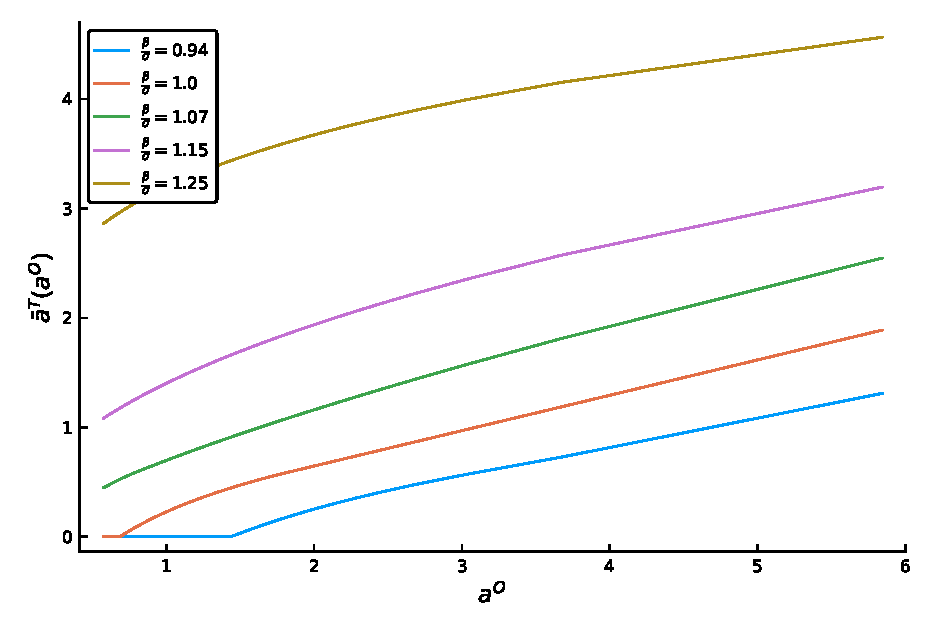
\includegraphics[width=.9\textwidth]{/Users/simeonalder/Dropbox/Work/Research/GitHub/teachers/julia/plots/occ_thresh_tauW_0.0_tauE_0.0_A=2.0.eps}
%\caption{ }
%\label{ }
\end{center}
\end{figure}
\end{frame}

\begin{frame}
\frametitle{Occupational Choice (Aggregate)}
\framesubtitle{Variation in Strength of Superstar Effect in Teaching: $\frac{\beta}{\sigma}$}
\begin{figure}
\begin{center}
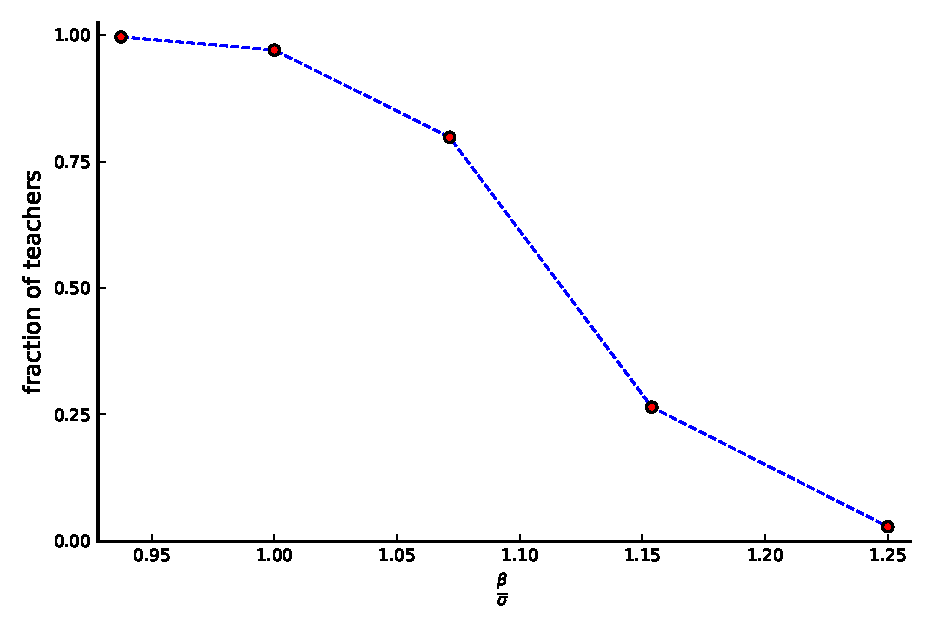
\includegraphics[width=.9\textwidth]{/Users/simeonalder/Dropbox/Work/Research/GitHub/teachers/julia/plots/frac_teachers_tauW_0.0_tauE_0.0_A=2.0.eps}
%\caption{ }
%\label{ }
\end{center}
\end{figure}
\end{frame}

\begin{frame}
\frametitle{Occupational Split}
\framesubtitle{Variation in Strength of Superstar Effect in Teaching: $\frac{\beta}{\sigma}$}
\begin{figure}
\begin{center}
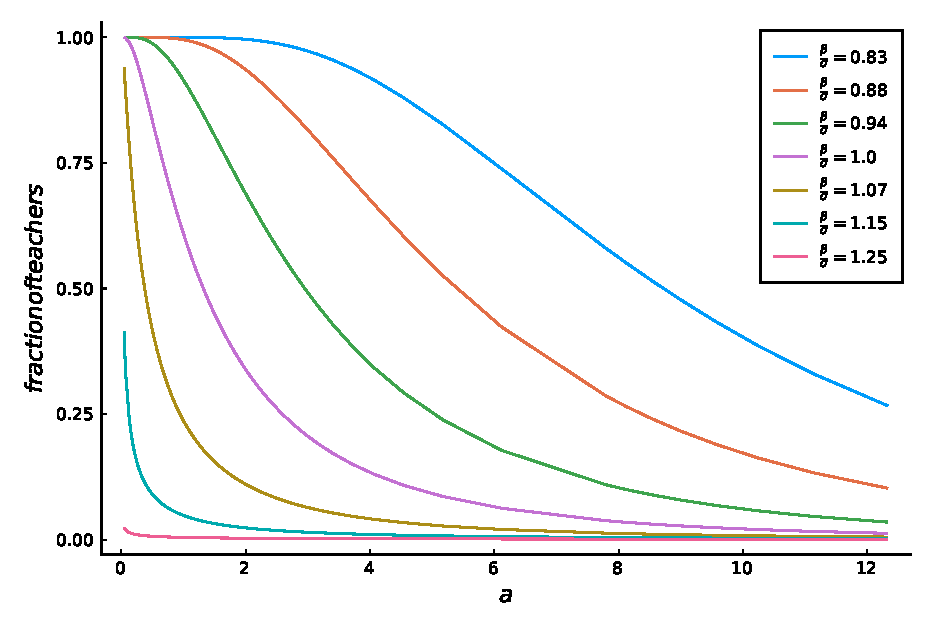
\includegraphics[width=.9\textwidth]{/Users/simeonalder/Dropbox/Work/Research/GitHub/teachers/julia/plots/frac_teachers_by_a_tauW_0.0_tauE_0.0_A=2.0.eps}
%\caption{ }
%\label{ }
\end{center}
\end{figure}
\end{frame}

\begin{frame}
\frametitle{Aggregate Law of Motion for $\widetilde{H^T}$}
\framesubtitle{Variation in Strength of Superstar Effect in Teaching: $\frac{\beta}{\sigma}$}
\begin{figure}
\begin{center}
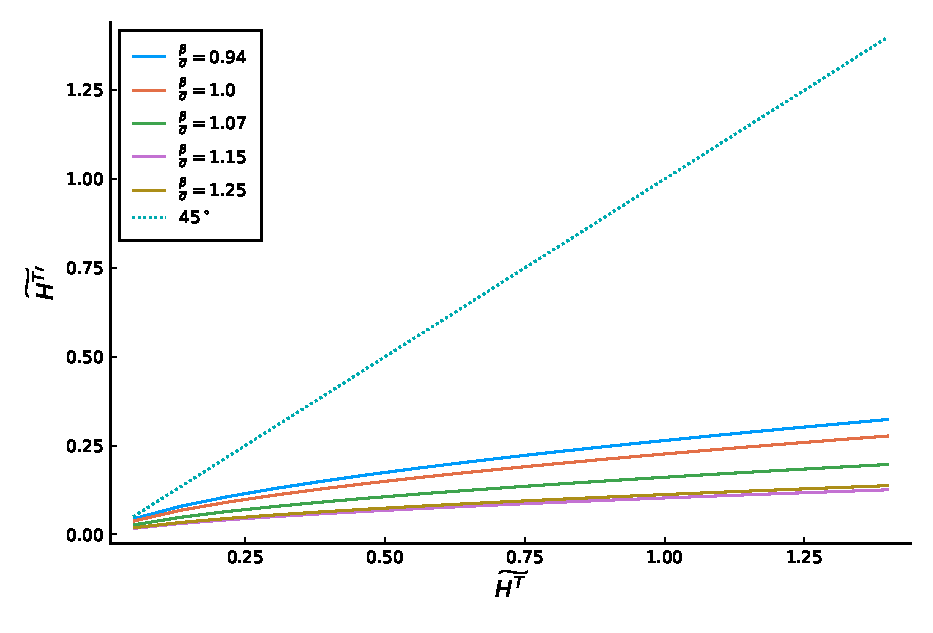
\includegraphics[width=.9\textwidth]{/Users/simeonalder/Dropbox/Work/Research/GitHub/teachers/julia/plots/law_of_motion_tauW_0.0_tauE_0.0_A=2.0.eps}
%\caption{ }
%\label{ }
\end{center}
\end{figure}
\end{frame}

\begin{frame}
\frametitle{Effect of $\tau^w$ on Occupational Choice}
\framesubtitle{$\frac{\beta}{\sigma} = 1.15$}
\begin{figure}
\begin{center}
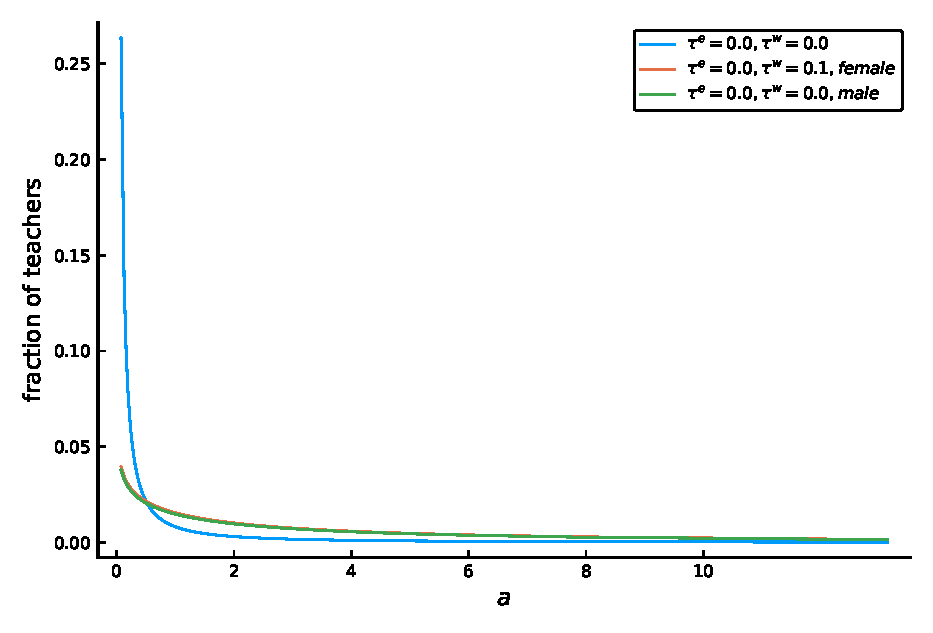
\includegraphics[width=.9\textwidth]{/Users/simeonalder/Dropbox/Work/Research/GitHub/teachers/julia/plots/frac_teachers_by_a_tauW_0.1_tauE_0.0_A=2.0.eps}
%\caption{ }
%\label{ }
\end{center}
\end{figure}
\end{frame}

\begin{frame}
\frametitle{Effect of $\tau^e$ on Occupational Choice}
\framesubtitle{$\frac{\beta}{\sigma} = 1.15$}
\begin{figure}
\begin{center}
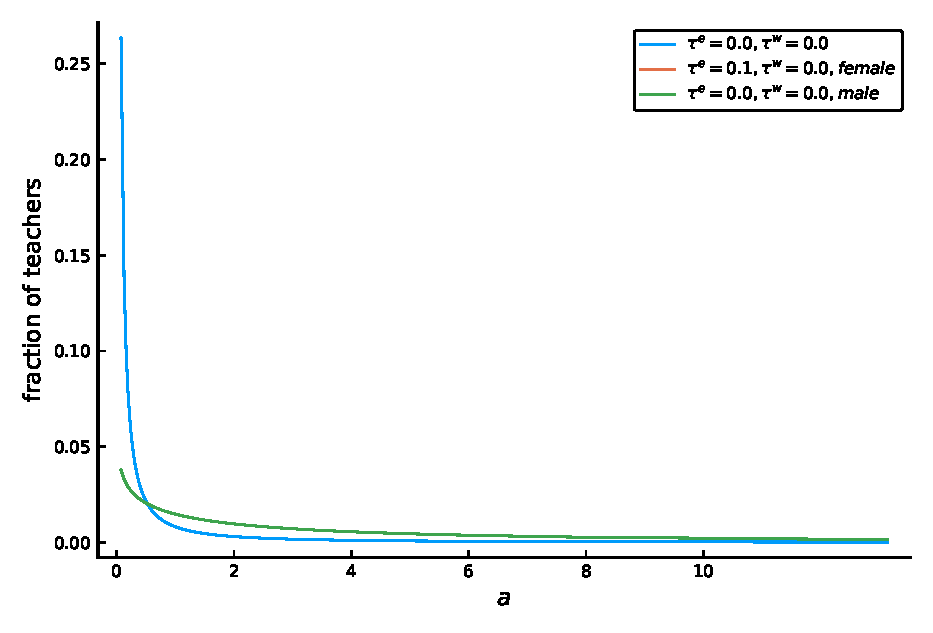
\includegraphics[width=.9\textwidth]{/Users/simeonalder/Dropbox/Work/Research/GitHub/teachers/julia/plots/frac_teachers_by_a_tauW_0.0_tauE_0.1_A=2.0.eps}
%\caption{ }
%\label{ }
\end{center}
\end{figure}
\end{frame}

\begin{frame}
\frametitle{Combined Effect of $\tau^w$ and $\tau^e$ on Occupational Choice}
\framesubtitle{$\frac{\beta}{\sigma} = 1.15$}
\begin{figure}
\begin{center}
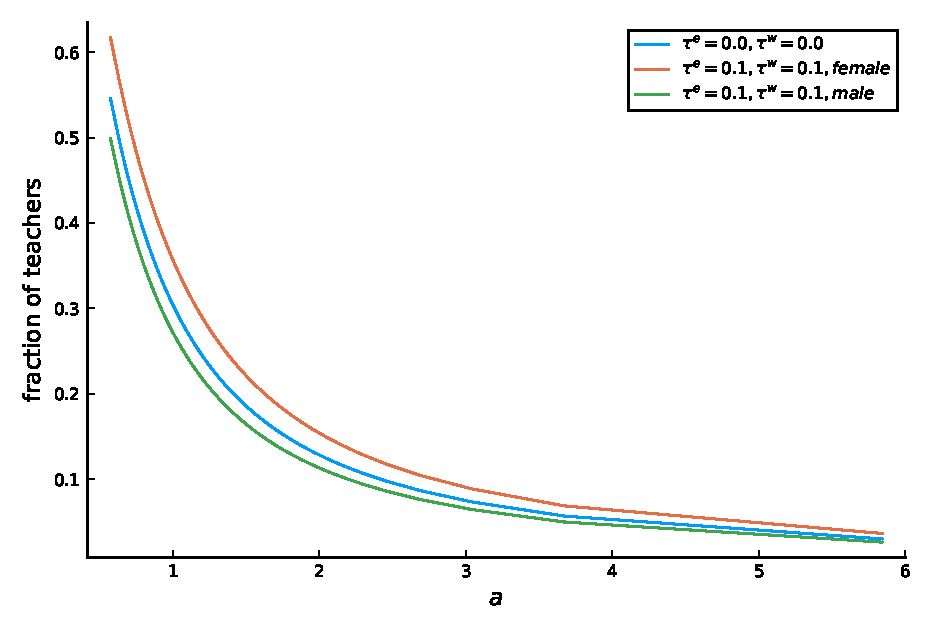
\includegraphics[width=.9\textwidth]{/Users/simeonalder/Dropbox/Work/Research/GitHub/teachers/julia/plots/frac_teachers_by_a_tauW_0.1_tauE_0.1_A=2.0.eps}
%\caption{ }
%\label{ }
\end{center}
\end{figure}
\end{frame}

\begin{frame}
\frametitle{Extensions}
\begin{itemize}
  \item Multiple locations:
  \begin{itemize}
  \item finite number of locations
  \item teachers' salaries funded by combination of local lump-sum (property) and proportional (sales) taxes
  \item one location with $T=0$, all locations have $t \in (0,1)$
  \item sorting of teachers and children into locations (high wage = high tax)
  \item sorting breaks global monotonicity between teacher's $h^T$ and class size (still holds locally, with random within-district assignment)
  \item to start with, solve with two locations (``high vs.~low'') 
  \end{itemize}
\end{itemize}
\end{frame}

\end{document}